\ifx\PREAMBLE\UnDef
\documentclass{beamer}
\usepackage{tikz}
\usepackage[english]{babel}
% or whatever

\usepackage[latin1]{inputenc}
% or whatever
\usepackage{xifthen}
\usepackage{bsymb}

\newcommand{\always}{\mathop{\square}}
\newcommand{\eventually}{\mathop{\diamondsuit}}
\newcommand{\until}{\mathop{\mathcal{U}}}

\begin{document}
\else
\fi

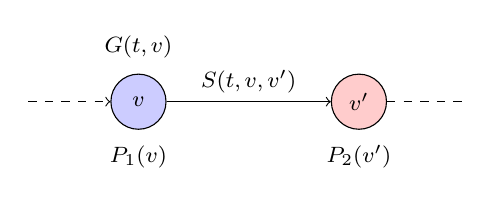
\begin{tikzpicture}[scale=0.7]
  \footnotesize
  \draw (2,0) node(s1)[circle, draw, inner sep =
  2pt, fill=blue!20!white, minimum width=0.7cm]{$v$};
  \draw (6,0) node(s2)[circle, draw, inner sep =
  2pt, fill=red!20!white, minimum width=0.7cm]{$v^\prime$};
  \draw[->, dashed] (0,0) -- (s1);
  \draw[->] (s1) --node[above]{$S(t,v,v^\prime)$} (s2);
  \draw[dashed] (s2) -- (8,0);
  \draw (2,1) node{$G(t,v)$};
  \draw (2,-1) node{$\structure{P_1(v)}$};
  \draw (6,-1) node{$\alert{P_2(v^\prime)}$};
\end{tikzpicture}

\ifx\PREAMBLE\UnDef
\end{document}
\else
\fi
